% Tento soubor nahraďte vlastním souborem s obsahem práce.
%=========================================================================
% Autoři: Michal Bidlo, Bohuslav Křena, Jaroslav Dytrych, Petr Veigend a Adam Herout 2019

% Pro kompilaci po částech (viz projekt.tex), nutno odkomentovat a upravit
%\documentclass[../projekt.tex]{subfiles}
%\begin{document}

\chapter{Úvod}

V~této práci se čtenář dozví informace o~hře Futoshiki, její pravidla
a~o~různých metodách, které slouží pro řešení této hry. Dále jsou v práci
zahrnuty také informace o~konečných automatech, které budou využity pro
vytvoření automatu řešitele hlavolamu.

V~první kapitole se tato práce zaměří na podrobný popis hry Futoshiki včetně
pravidel pro úspešné vyřešení. Dále budou v~této kapitole detailně popsány
algoritmy sloužící pro vyřešení mřížky Futoshiki, konkrétně algoritmy
Backtracking, Forward checking a~Arc Consistency \#3.

Třetí kapilota popíše existující konečné automaty, které jsou důležité pro
následnou derivaci automatu využitého pro řešení Futoshiki. Jsou zde popsány
deterministické a nedeterministické konečné automaty, dvojcestný konečný
automat, který nám ukáže základy dvojdimenzionálního automatu, a~nakonec také
skákající automat, na jehož definici bude z~velké části postavena definice
výsledného automatu pro řešení Futoshiki.

Ve čtvrté kapitole je popsán již výsledný automat, tedy dvojdimenzionální
skákájící automat, který umožňuje jak pohyb po mřížce ve čtyřech směrech,
stejně jako čtyřcestný automat, ale také skoky.

Následující kapitola obsahuje pravidla pro samotný automat. Jsou zde definovány
základní symboly a~následné řešení Futoshiki na základě jednotlivých algoritmů.
Algoritmy Forward checking a~Arc Consistency \#3 mnoho pravidel sdílí. Jsou to
například pravidla pro vytvoření domén a~základní pravidla řešení hry. To je
z~důvodu podobnosti algoritmů, kde Arc Consistency \#3 má pouze více striktní
úpravy domén.

Detailní popis implementace samotné je obsažen v kapitole šesté. Implementace
byla vyvinuta v~jazyce Rust s~pomocí knihovny termint. První část této kapitoly
se věnuje popisu spouštění aplikace. Jsou zde popsány veškeré argumenty pro
spuštění hry, ale také benchmarku nebo úpravy konfigurace. Následně je popsán
vzhled aplikace, která je implementována jako terminálová aplikace. Detailně
bude čtenář seznámen s~ovládáním aplikace, konkrétně s vyplňováním mřížky,
vytvářením mřížky a~s~ostatní funkcionalitou.

Poslední kapitola této práce se zaměří na testování. Hlavní důraz byl kladen
na správnost implementovaných algoritmů a~na jejich časovou náročnost. Čtenář
se dozví, jak se testovala správnost implementace jednotlivých částí aplikace,
tedy implementovaných algoritmů, ověřovače složení a~generátoru mřížky.
Následně bude popsáno testování časové náročnosti, které bylo provedeno pomocí
implementovaného benchmarku. Výsledek benchmarku, tedy graf obsahující průměrné
časy jednotlivých algoritmů pro mřížky od velikosti 4×4 až po velikost 10×10,
je také obsažen v~této kapitole.

\chapter{Futoshiki a algoritmy pro řešení}
\label{sec:futoshikiAlgs}

Tato kapitola se podrobně zaměřuje na pravidla hry Futoshiki a~algoritmy, které
jsou používány k~jejímu řešení. Nejprve se seznámíme s~pravidly, která jsou
nezbytná pro pochopení herních mechanismů, což nám umožní lépe porozumět
následně popsaným algoritmům pro řešení hlavolamu.

Prvním a~základním algoritmem, se kterým se seznámíme, je algoritmus
Backtracking. Tento algoritmus využívá princip systematického prozkoumávání
všech možných řešení metodou pokus-omyl. Ačkoli není nejefektivnější, poskytuje
klíčový základ pro pochopení dalších sofistikovanějších metod, které lze využít
k~řešení hlavolamu Futoshiki.

Následně se zaměříme na algoritmus Forward Checking a~jeho dvě možné
implementace. Tento algoritmus vylepšuje základní princip Backtrackingu tím, že
předběžně kontroluje možné hodnoty, což vede ke snížení počtu zkoušených
kombinací.

Nakonec bude popsáno možné vylepšení Forward Checkingu. Tento vylepšený
algoritmus se nazývá Arc Consistency \#3. Vylepšení spočívá ve více striktní
úpravě domén, což zabraňuje zbytečnému zkoušení hodnot, u~kterých je jasné, že
k~řešení nevede.

Všechny popsané algoritmy byly implementovány v~programu, který umožňuje řešení
libovolné mřížky hlavolamu Futoshiki. Implementace obsahuje i~benchmark, pomocí
kterého lze demonstrovat účinnost jednotlivých algoritmů v~různých herních
scénářích. Více o~benchmarku bude zmíněno v~sekci
\hyperref[sec:timeComplexity]{testování časové složitosti}.

\section{Pravidla hry}

Futoshiki \cite{FutoshikiWiki}, známá také jako hra "větší/menší" (More or
Less), je logický hlavolam pocházející z~Japonska, který je založen na podobném
principu jako sudoku. Hlavolam se skládá ze čtvercové mřížky, obvykle
o~velikosti 4x4, přičemž může být i~větší.

Pro úspěšné vyřešení je třeba každé pole v~mřížce vyplnit číslem od 1 do
velikosti mřížky. Dále musí platit pravidlo, že se v~každém řádku a~sloupci
čísla nesmí opakovat. Kromě toho jsou na mřížce umístěny nerovnosti mezi
některými poli, které určují vztah mezi dvěma čísly. Hra začíná s~libovolným
počtem již vyplněných polí a~nerovností, přičemž toto počáteční rozmístění musí
být v~souladu s~pravidly a~zaručovat existenci alespoň jednoho řešení. Následně
hráč vyplňuje zbývající pole, zatímco nerovnosti se již nemění a~nepřidávají se
žádné nové. Složená mřížka Futoshiki je takzvaný latinský čtverec
\cite{LatinSquareWiki}.

\section{Backtracking}

Backtracking \cite{PrednaskyIZU}\cite{BacktrackingWiki} je způsob řešení
algoritmických problémů, které jsou založeny na prohledávání stavového
prostoru. Je to jednoduchý a~často využívaný algoritmus, který systematicky
prohledává prostor řešení. Je založen na prohledávání do hloubky, tedy nejdříve
se zkusí celá cesta, než bude prohledáváno jiné řešení. Z~tohoto důvodu se
algoritmu Backtracking říká také metoda pokus-omyl - prohledá se jedna cesta
a~v~případě omylu se zkusí jiná.

\subsection{Postup algoritmu}

Postup Backtrackingu se může lišit v závislosti na řešeném problému.
Následující postup popisuje řešení mřížky Futoshiki. Na základě tohoto postupu
byla následně implementována rekurzivní varianta algoritmu.

\begin{enumerate}
    \item Posun na první nevyplněné pole. Pokud neexistuje, bylo nalezeno
        řešení.
    \item Postupné dosazování hodnot (1 až velikost mřížky) a~otestování, zda
        dosazená hodnota porušuje některé z~pravidel.
    \begin{enumerate}
        \item Pokud ano, zkouší se jiná hodnota.
        \item V opačném případě zápis hodnoty do pole a přesun na bod 1.
    \end{enumerate}
    \item Žádná hodnota nevede k řešení, zpětné navrácení na předchozí pole.
        Přesun na bod číslo 2, kdy se pokračuje v dosazování hodnot.
    \begin{enumerate}
        \item V případě, že neexistuje předchozí pole, řešení neexistuje.
    \end{enumerate}
\end{enumerate}

\subsection{Backtracking v praxi}

Algoritmus je velmi populární, jelikož lze využít pro řešení velkého množství
problémů a~jeho implementace je velice jednoduchá. Avšak kvůli jeho
exponenciální časové složitosti je vhodný pouze pro problémy, které mají malý
stavový prostor. To je dáno tím, že algoritmus zkouší všechny možnosti, bez
ohledu na to, zda je již z počátku zjevné, že daná možnost k~řešení nevede.

Nevýhoda tohoto algoritmu lze například pozorovat u~větších mřížek futoshiki.
Více o~jeho časové složitosti je popsáno v sekci
\hyperref[sec:timeComplexity]{testování časové složitosti}.

Z~tohoto důvodu se pro problémy s~velkými stavovými prostory využívají
algoritmy, které implementují další techniky k~zúžení stavového prostoru, čímž
se zlepšuje výpočetní náročnost. Tyto procedury pro zužování stavového prostoru
se nazývají look-ahead a~jsou popsány
v~\hyperref[sec:lookAhead]{následující sekci}.

\section{Look-ahead Backtracking}
\label{sec:lookAhead}

Pro optimalizaci algoritmu Backtracking se využívají procedury zvané
look-ahead \cite{LookAheadWiki}. Tato procedura se pokouší zmenšit stavový
prostor tím, že se pokusí předvídat účinky jednotlivých cest při hledání
řešení. Obecně algoritmy využívající této techniky uchovávají domény platných
hodnot u~každé proměnné. Tato doména se poté během provádění algoritmu mění na
základě predikcí.

Mezi algoritmy využívající look-ahead techniky patří například Forward Checking
a~Arc Consistency \#3.

\subsection{Heuristiky}

Algoritmy využívající technik look-ahead využívají heuristiky
\cite{PrednaskyIZU}, které dále optimalizují proces hledání řešení. Heuristika
určuje strategii výběru hracího pole a hodnoty, která bude dosazena do tohoto
pole. Existují dvě hlavní kategorie heuristik: heuristiky pro výběr hracího
pole a~heuristiky pro výběr hodnoty z~domény.

\subsubsection{Heuristiky výběru hracího pole}

Mezi heuristiky pro výběr hracího pole patří:

\begin{itemize}
    \item \textbf{Nejvíce omezená proměnná}: Tato heuristika vybírá hrací pole,
        které má nejmenší doménu, tedy pole, pro které je nejvíce omezený výběr
        možných hodnot.
    \item \textbf{Nejvíce omezující proměnná}: Heuristika volí hrací pole,
        které má největší vliv na omezení ostatních polí, tedy pole, které
        ovlivňuje nejvíce ostatních hodnot v~mřížce.
\end{itemize}

\subsubsection{Heuristiky výběru hodnoty z domény}

Mezi heuristiky pro výběr hodnoty z domény patří:

\begin{itemize}
    \item \textbf{Nejméně omezující hodnota}: Tato heuristika vybírá hodnotu,
        která má nejmenší vliv na ostatní domény. Tímto způsobem se
        minimalizuje riziko, že se algoritmus dostane do slepé uličky, když
        později dojdou možnosti pro jiná pole.
    \item \textbf{Náhodná hodnota}: Tento přístup vybírá hodnotu z domény
        náhodně.
\end{itemize}

\subsection{Ukládání domén}

Uložení domén může probíhat několika způsoby. Mezi klasické způsoby patří
ukládání hodnot do pole nebo seznamu, což však může být problematické, pokud
je potřeba efektivně vylučovat hodnoty z~domény nebo ověřovat, zda se hodnota
v~doméně nachází. Tento problém je způsoben nutností projít celé pole nebo
seznam, což je časově náročné. Tento problém lze vyřešit pomocí hašovacích
množin, které využívají hašovací tabulky. Ověření, zda se hodnota nachází
v~doméně, je efektivní s průměrnou časovou složitostí O(1), a~při mazání
hodnoty není třeba přeskupovat prvky, na rozdíl od běžného pole.

S rostoucí velikostí mřížky se zvyšuje i~využití paměti, kdy se při využití
hašovacích množin či polí jedná o~poměrně dost paměti. Efektivnější způsob
ukládání domén je možný pomocí bitmap, které vylepšují využití paměti tím, že
doménu reprezentují jako jedno číslo místo celého pole čísel. V~tomto případě
každé číslo v~doméně je reprezentováno jedním bitem. Jestliže je tedy v~doméně
obsaženo číslo 4, bit na čtvrté pozici bude nastaven na hodnotu 1. V~opačném
případě bude nastavet na hodnotu 0. Mezi nevýhody bitmap patří omezení
velikosti, které závisí na velikosti použitého datového typu. V~mé implementaci
jsem využil datový typ \texttt{usize}, kterého velikost závisí na architektuře
systému. Například na 64-bitovém procesoru má velikost 64 bitů.

Pro implementaci algoritmů s doménami jsem využil dva způsoby jejich ukládání:
pomocí hašovacích množin a~bitmap. Implementace je podobná, u~hašovacích množin
se využívají funkce pro práci s~množinami, zatímco u~bitmap se používají bitové
operace.

\subsection{Generování domén}

Při využití domén je na počátku algoritmu potřeba vygenerovat doménu pro každé
hrací pole. Generování domén lze implementovat více způsoby. Já je generuji ve
třech krocích:
\begin{enumerate}
    \item Generace domén řádků a~sloupců.
    \item Generace domén polí.
    \item Úprava domén na základě nerovností.
\end{enumerate}

\subsubsection{Generace domén řádků a sloupců}

Prvním krokem je generace domén řádků a sloupců. Ta se provádí iterací přes
všechny pole mřížky s~následným přidáváním hodnot, z~již vyplněných polí, do
domén daného řádku či sloupce.

\subsubsection{Generace domén polí}

Generování domén polí samotných probíhá v druhém kroku. Tato generace probíhá
na základě domén řádků a sloupců. Konkrétně je provedeno sjednocení domény
konkrétního řádku a~sloupce, čímž vznikne doména pro dané pole.

\subsubsection{Úprava domén na základě nerovností}

Posledním krokem v~generování je úprava domén polí ovlivněných nerovností.
Ta je provedena iterováním přes všechny nerovnosti a~následného úpravení domén
tak, aby obsahovaly pouze hodnoty, které by neporušily danou nerovnost.
Konkrétně z~domény pole, které má být menší, odstraním hodnoty, které jsou
větší nebo rovné maximální hodnotě z~domény druhého pole v~nerovnosti. Naopak
z~domény pole, které má být větší, budou odstraněny menší nebo rovné hodnoty
minimální hodnotě z~domény druhého pole v~nerovnosti.

\subsection{Forward Checking}
\label{sec:forwardChecking}

Forward Checking \cite{PrednaskyIZU} využívá již zmíněných look-ahead technik.
Tento algoritmus snižuje počet zkoušených kombinacích tím, že upravuje domény
všech přímo ovlivněných polí po zápisu do pole. Přímo ovlivněná pole v~případě
řešení Futoshiki taková pole, která se nachází ve stejném řádku či sloupci
a~nebo jsou v~nerovnosti s~polem, do kterého se zapisuje.

\subsubsection{Postup algoritmu}

Na základě následujícího postupu algoritmu Forward Checking pro řešení mřížky
Futoshiki byl algoritmus implementován. V~implementaci jsou poté pro výběr
hracího pole využil heuristiku nejvíce omezená proměnná. Z~domény tohoto pole
hodnoty vybírám postupně, nevyužívám tedy žádnou speciální heuristiku.

\begin{enumerate}
    \item Vygenerování domén pro každé pole a inicializace zásobníku stavů
        mřížky.
    \item Jestliže jsou všechna pole vyplněna, nalezeno řešení.
    \item Zvolení pole na základě heuristiky výběru hracího pole.
    \begin{enumerate}
        \item Jesliže doména je prázdná a~zásobník stavů mřížky je prázdný,
            neexistuje řešení.
        \item Jinak uložení aktuálního stavu mřížky.
    \end{enumerate}
    \item Zvolení hodnoty z~pole na základě heuristiky výběru hodnoty z~domény.
    \begin{enumerate}
        \item Odebrání zvolené hodnoty z~domény a~zápis hodnoty do pole.
        \item Úprava domén přímo ovlivněných polí.
        \item Přesun na bod číslo 2.
    \end{enumerate}
    \item Žádná z hodnot nevede k~řešení, obnovení a~odebrání stavu mřížky ze
        zásobníku a~přesun na bod číslo 3.
\end{enumerate}

\subsection{Arc Consistency \#3}

Algoritmus Arc Consistency \#3, známý také jako AC-3, rozšiřuje techniky
snižování zkoušených kombinací Forward Checkingu. AC-3 pracuje iterativně
s~množinou takzvaných oblouků (arc), kde každý oblouk reprezentuje vztah mezi
dvěma proměnnými. Algoritmus poté zajišťuje, aby během celého běhu byly všechny
domény konzistentní vzhledem ke všem omezením. Tento stav se nazývá Arc
Consistency.

Z~toho vyplývá, že po dosazení hodnoty do pole musí být upraveny všechny domény
přímo i~nepřímo ovlivněných polí. Přímo ovlivněná pole byla popsána v~sekci
o~\hyperref[sec:forwardChecking]{Forward Checkingu}. Nepřímo ovlivněná pole
jsou taková pole, která nejsou bezprostředně v~relaci se změněným polem, ale
změny se k~nim dostanou přes jiné proměnné. V~praxi to znamená, že změny se
propagují, dokud nenastane konzistentní stav, tedy dokud se mění domény.

\subsubsection{Postup algoritmu}

Na základě tohoto postupu byl algoritmus Arc Consistency \#3 implementován,
kde úprava domén nepřímo ovlivněných polí je implementována pomocí rekurze.
Jestliže dojde ke změně domény jsou upraveny i~všechny domény polí, které
vystupují v~nerovnosti s~upraveným polem. Tento postup se rekurzivně opakuje,
dokud se domény nepřestanou měnit a~tedy nedošlo ke konzistentního stavu.

Implementace využívá stejné heuristiky jako Forward Checking. Pro výběr
hracího pole je využita heuristiku nejvíce omezená proměnná. Z~domény tohoto
pole hodnoty vybírám postupně, nevyužívám tedy žádnou speciální heuristiku.

\begin{enumerate}
    \item Vygenerování domén pro každé pole a inicializace zásobníku stavů
        mřížky.
    \item Jestliže jsou všechna pole vyplněna, nalezeno řešení.
    \item Zvolení pole na základě heuristiky výběru hracího pole.
    \begin{enumerate}
        \item Jesliže doména je prázdná a~zásobník stavů mřížky je prázdný,
            neexistuje řešení.
        \item Jinak uložení aktuálního stavu mřížky.
    \end{enumerate}
    \item Zvolení hodnoty z~pole na základě heuristiky výběru hodnoty z~domény.
    \begin{enumerate}
        \item Odebrání zvolené hodnoty z~domény a~zápis hodnoty do pole.
        \item Úprava domén přímo i nepřímo ovlivněných polí.
        \item Přesun na bod číslo 2.
    \end{enumerate}
    \item Žádná z hodnot nevede k~řešení, obnovení a~odebrání stavu mřížky ze
        zásobníku a~přesun na bod číslo 3.
\end{enumerate}

\subsection{Look-ahead v praxi}

Využití look-ahead technik, jak už využitím algoritmu Forward Checking, tak
i~algoritmu Arc Consistency \#3, je velice užitečné. Díky těmto technikám se
stavový prostor může zúžit i~několikanásobně a~tím výrazně zlepšit výpočetní
rychlost.

Nevýhodou těchto technik je však potřebná režie, kdy čím pokročilejší techniky
jsou využity, tím více režie je potřeba. Z~tohoto důvodu se pro problémy
s~menším stavovým prostorem hodí algoritmu s~co nejmenší režií, jako je třeba
Backtracking. Tento problém lze velice dobře pozorovat při porovnávání
rychlosti složení různých velikostí mřížek Futoshiki se zmíněnými algoritmy.
Více o~tomto porovnání je popsáno v~sekci
\hyperref[sec:timeComplexity]{testování časové složitosti}.

\chapter{Existující formy konečných automatů}

\section{Konečný automat}

Konečné automaty jsou základní matematické modely sloužící k popisu a analýze
regulárních jazyků. Reprezentují abstraktní stroje, které zpracovávají vstupní
řetězce symbolů a rozhodují, zda patří do jazyka, který automat popisuje.
Rozlišujeme dva hlavní typy konečných automatů: deterministický konečný automat
(DKA), v němž každý stav má jednoznačně definovaný přechod pro každý symbol, a
nedeterministický konečný automat (NKA), jenž umožňuje více přechodů nebo i
jejich absenci pro konkrétní symbol. Oba typy mají stejný vyjadřovací
potenciál, protože každý nedeterministický konečný automat lze převést na
ekvivalentní deterministický.

\subsection{Deterministický konečný automat}

Deterministický konečný automat je pětice \((Q, \Sigma, \delta, q_0, F)\), kde:
\begin{itemize}
    \item \(Q\) je konečná neprázdná množina stavů.
    \item \(\Sigma\) je vstupní abeceda, konečná množina vstupních symbolů.
    \item \(\delta\) je přechodová funkce ve tvaru
        \(Q \times \Sigma \rightarrow Q\).
    \item \(q_0\) je počáteční stav, kde \(q_0 \in Q\).
    \item \(F\) je množina koncových nebo přijímacích stavů, kde
        \(F \subseteq Q\).
\end{itemize}

\subsection{Nedeterministický konečný automat}

Nedeterministický konečný automat je pětice \((Q, \Sigma,\delta, q_0, F)\),
kde:
\begin{itemize}
    \item \(Q\) je konečná neprázdná množina stavů.
    \item \(\Sigma\) je vstupní abeceda, konečná množina vstupních symbolů.
    \item \(\delta\) je přechodová funkce ve tvaru
        \(Q \times \Sigma \rightarrow Q\), kde \(\Sigma \cup \{\varepsilon\}\).
    \item \(q_0\) je počáteční stav, kde \(q_0 \in Q\).
    \item \(F\) je množina koncových nebo přijímacích stavů, kde
        \(F \subseteq Q\).
\end{itemize}

\subsection{Dvojcestný konečný automat}

Dvojcestné konečné automaty rozšiřují klasické konečné automaty tím, že čtecí
hlava se může pohybovat po vstupní pásce nejen zleva doprava, ale také zpět,
tedy doprava i doleva. To jim umožňuje prozkoumávat části vstupu vícekrát.
Stejně jako klasické konečné automaty se i dvojcestné konečné automaty dělí na
deterministické a nedeterministické.

I když dvojcestné automaty působí výkonněji než jednocestné automaty, mají
stejnou vyjadřovací sílu: přijímají pouze regulární jazyky. Tento výsledek
vychází z faktu, že každý dvojcestný konečný automat může být převeden na
ekvivalentní jednocestný automat (za cenu možného zvýšení počtu stavů).

Vstupní řetězec je ohraničen z obou stran speciálními symboly \{ |-, -| \},
které nejsou součástí vstupní abecedy \(\Sigma\). Tyto symboly slouží k
indikaci začátku a konce vstupu a čtecí hlava se za ně nesmí dostat. Pokud by
čtecí hlava narazila na jeden z těchto symbolů, automat zůstane na stejném
místě nebo přejde do koncového stavu.

\subsubsection*{Definice}

Dvojcestné konečné automaty jsou definované jako osmice
\((Q, \Sigma, |-, -|, \delta, s, t, r)\), kde:
\begin{itemize}
    \item \(Q\) je konečná množina stavů.
    \item \(\Sigma\) je konečná množina vstupních symbolů.
    \item |- je levý koncový symbol, přičemž platí \(|- \notin \Sigma\).
    \item -| je pravý koncový symbol, přičemž platí \(-| \notin \Sigma\).
    \item \(\delta\) je přechodová funkce ve tvaru \(Q \times (\Sigma \cup \{
        |-, -| \}) \rightarrow (Q \times \{ L, R \})\), přičemž \(L\) a \(R\)
        jsou směry pohybu čtecí hlavice.
    \item \(s\) je počáteční stav, kde \(s \in Q\).
    \item \(t\) je akceptující stav, kde \(t \in Q\).
    \item \(r\) je neakceptující stav, kde \(r \in Q\).
\end{itemize}

\subsection{Skákající automaty}

Skákající automat umožňuje čtecí hlavě skákat po vstupní pásce. Vstupní páska
je rozdělena do buněk, přičemž každá buňka obsahuje jeden symbol vstupního
řetězce. Automat čte symbol z buňky, na kterou ukazuje čtecí hlava, a na
základě aktuálního stavu a tohoto symbolu určuje, do jakého stavu přejde. Na
rozdíl od klasických konečných automatů, které se pohybují po pásce pouze zleva
doprava, může skákající automat přeskakovat mezi libovolnými buňkami. Pokud je
symbol již přečten, nemůže být přečten znovu.

\subsection{Skákající automat s opakovaným čtením}

\subsubsection*{Definice}

Skákající automat s opakovaným čtením lze definovat jako pětice
\(M = (Q, \Sigma, R, s F)\), kde:
\begin{itemize}
    \item \(Q\) je konečná množina stavů
    \item \(\Sigma\) je konečná množina vstupních symbolů
    \item \(R \subseteq Q \times \Sigma^* \times Q\) je konečná ternární
        relace, nazývaná množinou pravidel
        \begin{itemize}
            \item Každé pravidlo \((p, y, q) \in R\) je zapsáno jako
                \(py \rightarrow q\)
            \item Jestliže je aktuální stav automatu \(q\) a na vstupu je
                symbol odpovídající symbolu \(y\), automat přejde do stavu
                \(q\)
            \item Vstupní ukazatel zůstane na stejné pozici a nepřečte vstupní
                symbol
        \end{itemize}
    \item \(s \in Q\) je počáteční stav
    \item \(F \subseteq Q\) je množina konečných stavů
\end{itemize}

\subsubsection*{S podporou nerovností}

TEMP: definice stejná jako u skájícího automatu s opakovaným čtením. Změní se
pouze množina pravidel:

\begin{itemize}
    \item \(R \subseteq Q \times C(\Sigma^*) \times Q\)
    \begin{itemize}
        \item \(C\) je predikát, který musí být splněn aby proběhl přechod
        \item \(p[c] \rightarrow q\)
        \item \(p[x < 10] \rightarrow q\)
    \end{itemize}
\end{itemize}

\chapter{Dvojdimenzionální skákající automat}

Dvojdimenzionální skákající automaty jsou automaty, které vznikly spojením
dvou typů automatů - skákající a čtyřcestné automaty. Tento typ automatu je
díky skokům vhodný pro rychlejší procházení dvojrozměrné pásky. V~této práci
se skoky velice hodí pro rychlejší pohyb v~mřížce Futoshiki, bez kterých by
automat musel postupně mřížku procházet, dokud by nedošel na konkrétní pozici
ve vstupní pásce.

\section{Definice}

Sedmice \((Q, \Sigma, \Delta, R_1, R_2, s, F)\), kde:
\begin{itemize}
    \item \(Q\) je konečná množina stavů
    \item \(\Sigma\) je konečná množina vstupních symbolů
    \item \(\Delta\) je množina povolených směrů
    \item \(R_1\) množina pravidel pro pohyb ve tvaru
        \((Q \times \Sigma) \implies (Q \times \Delta)\)
    \item \(R_2\) množina pravidel pro skoky ve tvaru
        \(Q \implies (Q \times \Sigma)\)
    \item \(s \in Q\) je počáteční stav
    \item \(F \subseteq Q\) je množina konečných stavů
\end{itemize}

\chapter{Pravidla dvojdimenzionálního skákajícího automatu}

V~této kapitole se podrobně zaměříme na pravidla přechodů dvojdimenzionálního
skákajícího automatu, který je navrhnut pro řešení hlavolamu Futoshiki.
Nejdříve si definujeme základní značení, tedy abecedu symbolů a následně budou
obsažený pravidla pro jednotlivé algoritmy.

\section{Základní značení}

\begin{itemize}
    \item \(\#\#\) - hranice hrací mřížky
    \item \(\#\) - hranice mezi hracími poli
    \item \(N\) - nerovnost mezi poli
    \item \(N_-\) - horizontální nerovnost mezi poli
    \item \(N_|\) - vertikální nerovnost mezi poli
    \item \(F\) - vyplněné herní pole
    \item \(X\) - nevyplněné herní pole
    \item \(\{X\}\) - pole s~neprázdnou doménou
    \item \(\{L\}\) - pole s~nejmenší doménou
    \item \(\{\}\) - pole s~prázdnou doménou
    \item \(E\) - pole bez domény
    \item \(R\), \(L\), \(U\), \(D\) - směry pohybu v~mřížce
\end{itemize}

\section{Pravidla pro Backtracking}

\begin{tabular}{@{}p{4cm} p{10.5cm}@{}}
    \(Q_{0} \implies Q_{10}X\) & Skok na první nevyplněné pole \\
    \(Q_{0} \implies Q_{F}\) & Všechna pole jsou vyplněná, přesun do koncového
        stavu \\

    & \\
    \(Q_{10} \implies Q_{11}U\) & Uložení jedné z možných hodnot na zásobník \\
    \(Q_{11}\#\# \implies Q_{12}D\) & Konec mřížky, posun dolů a přesun do
        stavu kontroly výskytu zapsané hodnoty \\
    \(Q_{11} \implies Q_{11}U\) & Jinak posun nahoru \\
    \(Q_{12}F \implies Q_{12}D\) & TODO: ověření existence \\
    \(Q_{12}\#\# \implies Q_{13}U\) & Konec mřížky, přesun do stavu vrácení
        na původní pole \\
    \(Q_{12} \implies Q_{12}D\) & Jinak posun dolů \\
    \(Q_{13} \implies Q_{14}X\) & Skok na původní pole, přesun do stavu
        horizontálního ověření \\

    & \\
    \(Q_{14}\#\# \implies Q_{15}R\) & Konec mřížky, posun doprava a přesun do
        stavu kontroly výskytu zapsané hodnoty \\
    \(Q_{14} \implies Q_{14}L\) & Jinak posun doleva \\
    \(Q_{15}F \implies Q_{15}R\) & TODO: ověření existence \\
    \(Q_{15}\#\# \implies Q_{20}L\) & Konec mřížky, přesun do stavu ověření
        nerovností \\
    \(Q_{15} \implies Q_{15}R\) & Jinak posun doprava \\

    & \\
    \(Q_{20} \implies TODO\) & Ověření nerovností \\
\end{tabular}

\section{Vytvoření domén polí}

\subsection*{Pravidla}

\subsubsection*{Vytvoření domén řádků a sloupců}

\begin{tabular}{@{}p{4cm} p{10.5cm}@{}}
    \(Q_0\#\# \implies Q_{01}R\) & Posun doprava pro vynechání okraje mřížky \\
    \(Q_{01}\#\# \implies Q_{11}D\) & Posun dolů pro vynechání okraje mřížky \\

    & \\
    \(Q_{10}\#\# \implies Q_{19}R\) & Posun doprava a~přesun do stavu
        ověření konce mřížky \\
    \(Q_{11}F \implies Q_{11}R\) & Odstranění hodnoty z~domény řádku a~sloupce
        a~posun doprava \\
    \(Q_{11}\#\# \implies Q_{20}D\) & Posun dolů pokud hranice mřížky \\
    \(Q_{11} \implies Q_{11}R\) & Jinak posun doprava \\
    \(Q_{19}\# \implies Q_{11}D\) & Následuje další řádek, přesun do stavu
        úpravy domén \\
    \(Q_{19} \implies Q_{39}U\) & Konec mřížky, přesun do stavu
        vytvoření domén polí \\

    & \\
    \(Q_{20}\#\# \implies Q_{29}L\) & Posun doleva a~přesun do stavu ověření
        konce mřížky \\
    \(Q_{21}F \implies Q_{21}L\) & Odstranění hodnoty z~domény řádku a~sloupce
        a~posun doleva \\
    \(Q_{21}\#\# \implies Q_{10}D\) & Posun dolů pokud hranice mřížky \\
    \(Q_{21} \implies Q_{21}L\) & Jinak posun doleva \\
    \(Q_{29}\# \implies Q_{21}D\) & Následuje další řádek, přesun do stavu
        úpravy domén \\
    \(Q_{29} \implies Q_{49}U\) & Konec mřížky, přesun do stavu
        vytvoření domén polí \\
\end{tabular}

\subsubsection*{Vytvoření domén polí}

\begin{tabular}{@{}p{4cm} p{10.5cm}@{}}
    \(Q_{30}\#\# \implies Q_{39}R\) & Posun doprava a~přesun do stavu ověření
        konce mřížky \\
    \(Q_{31}E \implies Q_{31}R\) & Vytvoření domény na základě domén řádku
        a~sloupce \\
    \(Q_{31}\#\# \implies Q_{40}U\) & Posun nahoru pokud hranice mřížky \\
    \(Q_{31} \implies Q_{31}R\) & Jinak posun doprava \\
    \(Q_{39}\# \implies Q_{31}L\) & Existuje předchozí řádek, přesun do stavu
        vytváření domén polí \\
    \(Q_{39} \implies Q_{50}\) & Konec mřížky, přesun do stavu úpravy domén na
        základě nerovností \\

    & \\
    \(Q_{40}\#\# \implies Q_{49}L\) & Posun doleva a~přesun do stavu ověření
        konce mřížky \\
    \(Q_{41}E \implies Q_{41}L\) & Vytvoření domény na základě domén řádku
        a~sloupce \\
    \(Q_{41}\#\# \implies Q_{30}U\) & Posun nahoru pokud hranice mřížky \\
    \(Q_{41} \implies Q_{41}L\) & Jinak posun doleva \\
    \(Q_{49}\# \implies Q_{41}U\) & Existuje předchozí řádek, přesun do stavu
        vytváření domén polí \\
    \(Q_{49} \implies Q_{50}\) & Konec mřížky, přesun do stavu úpravy domén na
        základě nerovností \\
\end{tabular}

\subsubsection*{Úprava domén na základě nerovností}

\begin{tabular}{@{}p{4cm} p{10.5cm}@{}}
    \(Q_{50} \implies Q_{51}N_-\) & Skok na horizontální nerovnost \\
    \(Q_{50} \implies  Q_{60}\) & Žádná další horizontální nerovnost, přesun do
        stavu prohledávání vertikálních nerovností \\
    \(Q_{51} \implies Q_{52}L\) & Posun doleva na první pole v~nerovnosti,
        uložení domény \\
    \(Q_{52} \implies Q_{53}R\) & Posun zpět na nerovnost \\
    \(Q_{53} \implies Q_{54}R\) & Posun doprava na druhé pole v~nerovnosti,
        uložení domény \\
    \(Q_{54} \implies Q_{55}L\) & Posun zpět na nerovnost, úprava domén na
        základě nerovnosti \\

    & \\
    \(Q_{60} \implies Q_{61}N_|\) & Skok na vertikální nerovnost \\
    \(Q_{60} \implies Q_{70}\) & Žádná další vertikální nerovnost, přesun do
        stavu řešení hry \\
    \(Q_{61} \implies Q_{62}U\) & Posun nahoru na první pole v~nerovnosti,
        uložení domény \\
    \(Q_{62} \implies Q_{63}D\) & Posun zpět na nerovnost \\
    \(Q_{63} \implies Q_{64}D\) & Posun dolů na druhé pole v~nerovnosti,
        uložení domény \\
    \(Q_{64} \implies Q_{65}U\) & Posun zpět na nerovnost, úprava domén na
        základě nerovnosti \\
\end{tabular}

\section{Řešení hry}

Pravidla pro řešení hry

\subsection*{Pravidla}

\begin{tabular}{@{}p{4cm} p{10.5cm}@{}}
    \(Q_{70} \implies Q_{71}\{L\}\) & Skok na pole s nejmenší doménou \\
    \(Q_{71}{} \implies Q_{BT}U\) & Nefunkční řešení, vrácení do řešitelného
        stavu \\
    \(Q_{71} \implies Q_{72}U\) & Jinak zvolení hodnoty z domény a přesun do
        stavu odstranění hodnoty z ovlivněných domén \\
    \(Q_{72}\#\# \implies Q_{73}D\) & Posun zpět do herního pole \\
    \(Q_{72} \implies Q_{72}U\) & Jinak posun nahoru \\

    \(Q_{73}X \implies Q_{73}D\) & Odstranění hodnoty z domény a posun dolů \\
    \(Q_{73}\#\# \implies Q_{74}\) & Konec mřížky, přesun do stavu odstraňování
        hodnot z domén horizontálních sousedů \\
    \(Q_{73} \implies Q_{73}D\) & Jinak pouze posun dolů \\

    \(Q_{74} \implies Q_{75}\{L\}\) & Skok na pole s nejmenší doménou \\
    \(Q_{75}\#\# \implies Q_{76}R\) & Posun zpět do herního pole \\
    \(Q_{75} \implies Q_{75}L\) & Jinak posun doleva \\

    \(Q_{76}X \implies Q_{76}R\) & Odstranění hodnoty z domény a posun
        doprava \\
    \(Q_{76}\#\# \implies Q_{77}\) & Konec mřížky, přesun do stavu zapsání
        hodnoty do pole \\
    \(Q_{76} \implies Q_{76}R\) & Jinak pouze posun doprava \\

    \(Q_{77} \implies Q_{70}\{L\}\) & Skok zpět na pole s nejmenší doménou a
        zapsání hodnoty \\
\end{tabular}

\chapter{Implementace}

Tato kapitola podrobně popisuje implementaci aplikace pro řešení hry Futoshiki.
V~rámci řešení jsou využity algoritmy uvedené v~kapitole
\hyperref[sec:futoshikiAlgs]{futoshiki a algoritmy pro řešení}.

V~první části bude čtenář seznámen se spouštěním aplikace, konkrétně
s~veškerými podporovanými argumenty pro spuštění, díky kterým lze aplikaci
před spuštěním nakonfigurovat.

Podrobně je také popsáno uživatelské prostředí aplikace, která je vytvořena
jako terminálová aplikace, tedy veškeré prvky rozhraní jsou zobrazeny pomocí
textu vytištěného do terminálu.

Nakonec bude popsán formát souboru konfigurace, který umožňuje nastavit výchozí
hodnoty argumentů pro spuštění aplikace.

Aplikace je implementována v~programovacím jazyce Rust za využití knihovny
\texttt{termint}, která zjednodušuje tvorbu uživatelského rozhraní v~terminálu.
Vývoj probíhal na operačním systému Linux.

\section{Spuštění aplikace}

Pomocí argumentů lze při spouštění aplikace upřesnit, jaká část implementace
má být spuštěna. Aplikace podporuje tři druhy spuštění:
\begin{enumerate}
    \item Spuštění hry
    \item Spuštění benchmarku
    \item Úprava výchozí konfigurace
\end{enumerate}

\subsection*{Argumenty pro spuštění hry}

Výchozím druhem spuštění aplikace je spuštění hry. Pro tento typ spuštění není
vyžadován žádný dodatečný argument. Dostupné argumenty jsou:

\begin{itemize}
    \item \texttt{-s, --size [číslo]}: Nastaví velikost mřížky (výchozí je 4)
    \item \texttt{--solver [typ]}: Zvolí algoritmus pro řešení Futoshiki
        (\hyperref[sec:argsAlgs]{dostupné algoritmy})
    \item \texttt{-t, --theme [téma]}: Téma aplikace (jak aplikace vypadá)
    \begin{itemize}
        \item \texttt{light}: Světlé téma
        \item \texttt{dark}: Tmavé téma
        \item \texttt{default}: Výchozí téma
    \end{itemize}
\end{itemize}

\subsection*{Argumenty pro benchmark}

Pro přepnutí spuštění na benchmark je potřeba využít argument \texttt{bench},
za kterým mohou být následující argumenty:

\begin{itemize}
    \item \texttt{-s, --size [číslo]}: Nastaví velikost testované mřížky, lze
        zadat vícekrát
    \item \texttt{--solver [typ]}: Zvolí testovaný algoritmus, lze zadat
        vícekrát (\hyperref[sec:argsAlgs]{dostupné algoritmy})
    \item \texttt{-r, --repeats [číslo]}: Nastaví počet opakování testu
    \item \texttt{-b, --boards [číslo]}: Nastaví počet testovaných mřížek
\end{itemize}

\subsection*{Dostupné typy algoritmů}
\label{sec:argsAlgs}

Argumenty vyžadující typ algoritmu podporují následující hodnoty:

\begin{itemize}
    \item \texttt{bt, backtrack, backtracking}: Backtracking
    \item \texttt{fc, forward-check, forward-checking}: Forward Checking
    \item \texttt{fcb, forward-check-bit, forward-checking-bit}: Forward
        Checking s~bitovými operacemi
    \item \texttt{ac3, arc-cons3, arc-consistency3}: Arc Consistency \#3
    \item \texttt{ac3b, arc-cons3-bit, arc-consistency3-bit}: Arc Consistency
        \#3 s~bitovými operacemi
\end{itemize}

\subsection*{Argumenty konfigurace}

Pokud je aplikace spuštěna s~argumentem \texttt{config}, otevře se konfigurační
soubor ve výchozím textovém editoru. Jestliže soubor neexistuje, automaticky se
vytvoří. Formát konfiguračního souboru je detailně popsán v~sekci
\hyperref[sec:appConfig]{konfigurace aplikace}.

\section{Vzhled a možnosti aplikace}

Po spuštění hry se zobrazí mřížka Futoshiki, která má čtvercový tvar s~předem
nastavenou velikostí. V~této mřížce je jedno z~polí zvýrazněno, to značí právě
označené pole. Pro změnu označeného pole lze využít klávesy šipek nebo klávesy
\texttt{hjkl}, které využívá textový editor \texttt{Vim} pro navigaci v~textu.
Aplikaci lze kdykoliv ukončit stiskem kláves \texttt{Q} a~\texttt{Esc}.
Aplikace obsahuje tři stránky:
\begin{enumerate}
    \item Vytváření mřížky
    \item Řešení mřížky
    \item Změna řešícího algoritmu
\end{enumerate}

\begin{figure}[hbt]
	\centering
	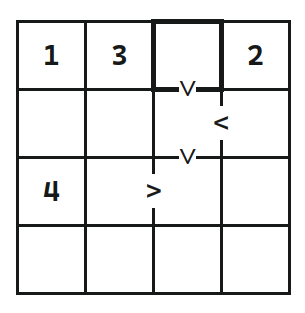
\includegraphics[width=0.4\textwidth]{obrazky-figures/futoshiki.png}
	\caption{Vzhled aplikace po spuštění hry se světlým tématem}
	\label{futoshiki}
\end{figure}

\subsection{Vytváření mřížky}

Tato stránka umožňuje uživateli vytvořit vlastní mřížku, kterou lze následně
nechat složit jedním z~algoritmů. Na tuto stránku se lze dostat ze stránky hry
stisknutím klávesy \texttt{B}. Pro následné vrácení na stránku hry lze opět
stisknout klávesu \texttt{B}.

\subsection*{Funkcionalita}
\begin{enumerate}
    \item Přidání hodnoty:
    \begin{itemize}
        \item Napsáním číselné hodnoty na klávesnici se hodnota přidá do
            označeného pole.
        \item Pokud hodnota přesáhne maximální povolenou hodnotu, odstraní
            se číslice z vyšších řádů.
    \end{itemize}
    \item Smazání hodnoty:
    \begin{itemize}
        \item Hodnotu lze smazat zapsáním čísla nula nebo klávesou
            \texttt{Delete}.
        \item Stiskem klávesy \texttt{Backspace} bude odstaněna číslice z~řádu
            jednotek.
    \end{itemize}
    \item Přidání nerovnosti:
    \begin{itemize}
        \item Právě označené pole bude prvním prvek nerovnosti.
        \item Stisknutím klávesy \texttt{>} (větší) nebo \texttt{<} (menší) se
            vybere typ nerovnosti.
        \item Zvolením sousedního pole se nastaví druhý prvek nerovnosti
            a~přidá se samotná nerovnost.
    \end{itemize}
    \item Smazání nerovnosti:
    \begin{itemize}
        \item Postup je stejný jako při přidávání nerovnosti, pouze místo
        kláves \texttt{>} nebo \texttt{<} se použije klávesa \texttt{C}.
    \end{itemize}
\end{enumerate}

\subsection*{Spuštění řešení}

Po dokončení vytváření mřížky lze stisknutím klávesy \texttt{S} aktivovat
aktuálně zvolený algoritmus, který následně mřížku vyřeší. V případě úspěchu
se do mřížky doplní zbývající hodnoty a~nad mřížku se vypíše zpráva o~úspešném
složení. V opačném případě bude nad mřížku vypsaná zpráva, že mřížka není
složitelná.

\subsection{Řešení mřížky}

Tato stránka umožňuje mřížku Futoshiki řešit. Uživateli však neumožňuje
odstraňovat hodnoty vložené již z~počátku a~také upravovat nerovnosti.

\subsection*{Funkcionalita}
\begin{enumerate}
    \item Generování mřížky:
    \begin{itemize}
        \item Stisknutím klávesy \texttt{Enter} se vygeneruje náhodná mřížka.
    \end{itemize}
    \item Řešení mřížky:
    \begin{itemize}
        \item Hodnoty lze do polí zapisovat stejným způsobem jako při vytváření
            mřížky.
        \item Nelze přepisovat hodnoty, které byly vygenerovány a~nelze měnit
            nerovnosti.
    \end{itemize}
\end{enumerate}

\subsection*{Dokončení řešení}

Jestliže je mřížka úspěšně vyřešena, zobrazí se zpráva o~úspěšném složení.
Pokud má uživatel problém se složením mřížky, lze opět využít nastaveného
algoritmu stisknutím klávesy \texttt{S} a~tím zobrazit správné řešení.

\subsection{Změna řešícího algoritmu}

Poslední stránkou v implementaci je stránka změny řešícího algoritmu. Díky
této stránce nemusí uživatel hru zavírat a spouštět znovu s odpovídajícími
argumenty, jenom aby změnil řešící algoritmus.

\begin{enumerate}
    \item Přechod mezi stránkou výběru a stránkou hry:
    \begin{itemize}
        \item Stisknutím klávesy \texttt{Tab} se přepne stránka.
        \item Pokud je aktuální stránka hra, přepne se na stránku výběru,
            v~opačném případě se přejde na stránku hry.
    \end{itemize}
    \item Výběr algoritmu:
    \begin{itemize}
        \item Výběr lze měnit pomocí kláves šipka nahoru a šipka dolů.
        \item Pro potvrzení výběru je třeba stisknout klávesu \texttt{Enter}.
            Zároveň se automaticky přejde na stránku hry.
    \end{itemize}
\end{enumerate}

\begin{figure}[hbt]
	\centering
	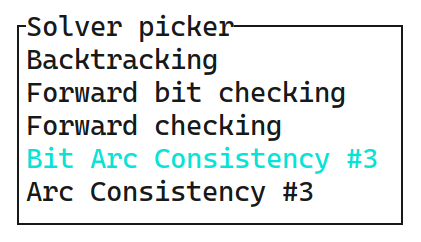
\includegraphics[width=0.6\textwidth]{obrazky-figures/solvers.png}
	\caption{Stránka výběru řešícího algoritmu}
	\label{solvers}
\end{figure}

\section{Konfigurace aplikace}
\label{sec:appConfig}

V případě, že uživatel spouští opakovaně aplikaci se stejnými argumenty, je
vhodné si nastavit výchozí hodnoty argumentů v konfiguračním souboru. Ten je
ve formátu JSON a obsahuje následující pole:

\begin{center}
    \begin{tabularx}{0.65\textwidth}{|l|l|X|}
        \hline
        \textbf{Název} & \textbf{Typ} & \textbf{Popis} \\
        \hline
        \texttt{defaultSize} & Integer & Výchozí velikost mřížky \\
        \hline
        \texttt{defaultSolver} & String & Výchozí řešící algoritmus \\
        \hline
        \texttt{defaultTheme} & String & Téma uživatelské aplikace \\
        \hline
    \end{tabularx}
\end{center}

Konfigurační soubor by pak mohl vypadat například takto:

\begin{verbatim}
{
    "defaultSize": 10,
    "defaultSolver": "ArcConsistency3Bit",
    "defaultTheme": "Light"
}
\end{verbatim}

\chapter{Testování}

Tato kapitola se zaměřuje na testování aplikace, především na ověření
správnosti a~výkonnosti implementovaných algoritmů. Testování zahrnuje kontrolu
správnosti výsledků algoritmů, aby byla zajištěna jejich funkčnost při řešení
hry Futoshiki. Současně je hodnocena časová náročnost algoritmů, přičemž jejich
výkonnost je porovnána při různých velikostech hrací mřížky.

\section{Správnost řešení}

Při testování správnosti řešení se zaměřuji na několik klíčových částí
aplikace: samotné algoritmy, ověřovač složení a~proces generování mřížky.

\subsection*{Testování algoritmů}

Pro testování algoritmů jsem vygeneroval čtyři různé mřížky s~různými úrovněmi
obtížnosti ze stránky futoshiki.com \cite{FutoshikiCom}. Každý algoritmus tyto
mřížky vyřešil a~výsledky byly následně zkontrolovány pomocí ověřovače složení,
který zajišťuje, že výsledná mřížka splňuje pravidla Futoshiki.

\subsection*{Testování ověřovače složení}

Ověřovač složení byl testován na mřížkách vygenerovaných ze stránky
futoshiki.com \cite{FutoshikiCom}, které byly předem složeny. Pro ověření
správnosti jsem u~některých mřížek pozměnil jejich řešení tak, aby obsahovaly
chyby. Tímto způsobem jsem testoval schopnost ověřovače určit, zda je mřížka
správně složena či nikoli.

\subsection*{Testování generování mřížky}

V~testovacím procesu generování mřížek bylo nejdříve vytvořeno několik
náhodných mřížek, které byly následně složeny pomocí jednoho z~algoritmů.
Výsledné složené mřížky byly zkontrolovány ověřovačem složení, což zajišťuje,
že každá vygenerovaná mřížka je řešitelná a~splňuje pravidla hry.

\section{Časová náročnost}
\label{sec:timeComplexity}

Testování časové náročnosti je prováděno po spuštění aplikace s~argumentem
\texttt{bench}. Tento režim umožňuje měřit výkonnost zvolených algoritmů (při
výchozím nastavení všech algoritmů) na různých velikostech mřížek.

Pro každou velikost mřížky je náhodně vygenerována mřížka, kterou následně
vyřeší každý algoritmus. Aby se minimalizoval vliv náhodných výkyvů, je test
opakován předem nastaveným počtem iterací (výchozí hodnota je 10). Pro každou
velikost mřížky je navíc test proveden na nastaveném počtu mřížek (výchozí
hodnota je 1). Po dokončení testování aplikace zobrazí v~terminálu výsledky
obsahující nejlepší, průměrný a~nejhorší naměřený čas pro každý algoritmus
a~velikost mřížky.

Kromě textového výstupu aplikace automaticky generuje graf, který vizualizuje
průměrné časy jednotlivých algoritmů pro různé velikosti mřížek. Tento graf
usnadňuje porovnání efektivity algoritmů při řešení s~různě velkými mřížkami.

\begin{figure}[hbt]
	\centering
	
\includegraphics[width=1\textwidth]{obrazky-figures/benchmark.png}
	\caption{
        Srovnání časové náročnosti všech algoritmů při různých velikostech
        mřížky (4×4 až 10×10).
    }
	\label{benchmark}
\end{figure}

\subsection{Zhodnocení}

Jak ukazuje graf, menší mřížky zvládnou všechny algoritmy rychle. Backtracking
je však nejrychlejší a~to díky své jednoduchosti a~absenci režie, jako je
generování domén polí. S~rostoucí velikostí mřížky však jeho výkon výrazně
klesá, což je dáno jeho systematickým prohledáváním všech možností, kdy počet
možností, které je třeba vyzkoušet, exponenciálně roste.

Na větších mřížkách jsou rozdíly mezi algoritmy výraznější. Je také důležité
zmínit, že osa \texttt{y}~je logaritmická, což může zkreslovat reálně rozdíly.
Backtracking je při velikosti 10×10 pomalejší přibližně o~deset sekund než
další nejpomalejší algoritmus. Nejlépe si vedly algoritmy Forward Checking
a~Arc Consistency \#3 a~to v~jejich implementaci s~bitmapami.

\chapter{Závěr}

%===============================================================================

% Pro kompilaci po částech (viz projekt.tex) nutno odkomentovat
%\end{document}
